%%%%%%%%                       01 - Motivation                      %%%%%%%%
%---------------------------------------------------------------------------
% 5 minutes total: keep each slide to 2--3 points.
%---------------------------------------------------------------------------

\begin{frame}
  \frametitle{Motivation}
  \begin{columns}
    \column{0.46\textwidth}
    \begin{itemize}
        \item Distributed control systems are hard to prototype \& debug.
        \item Goal: a lightweight runtime that executes communicating timed automata.
        \item Same model, multiple nodes, observable behaviour.
    \end{itemize}

    \column{0.54\textwidth}
    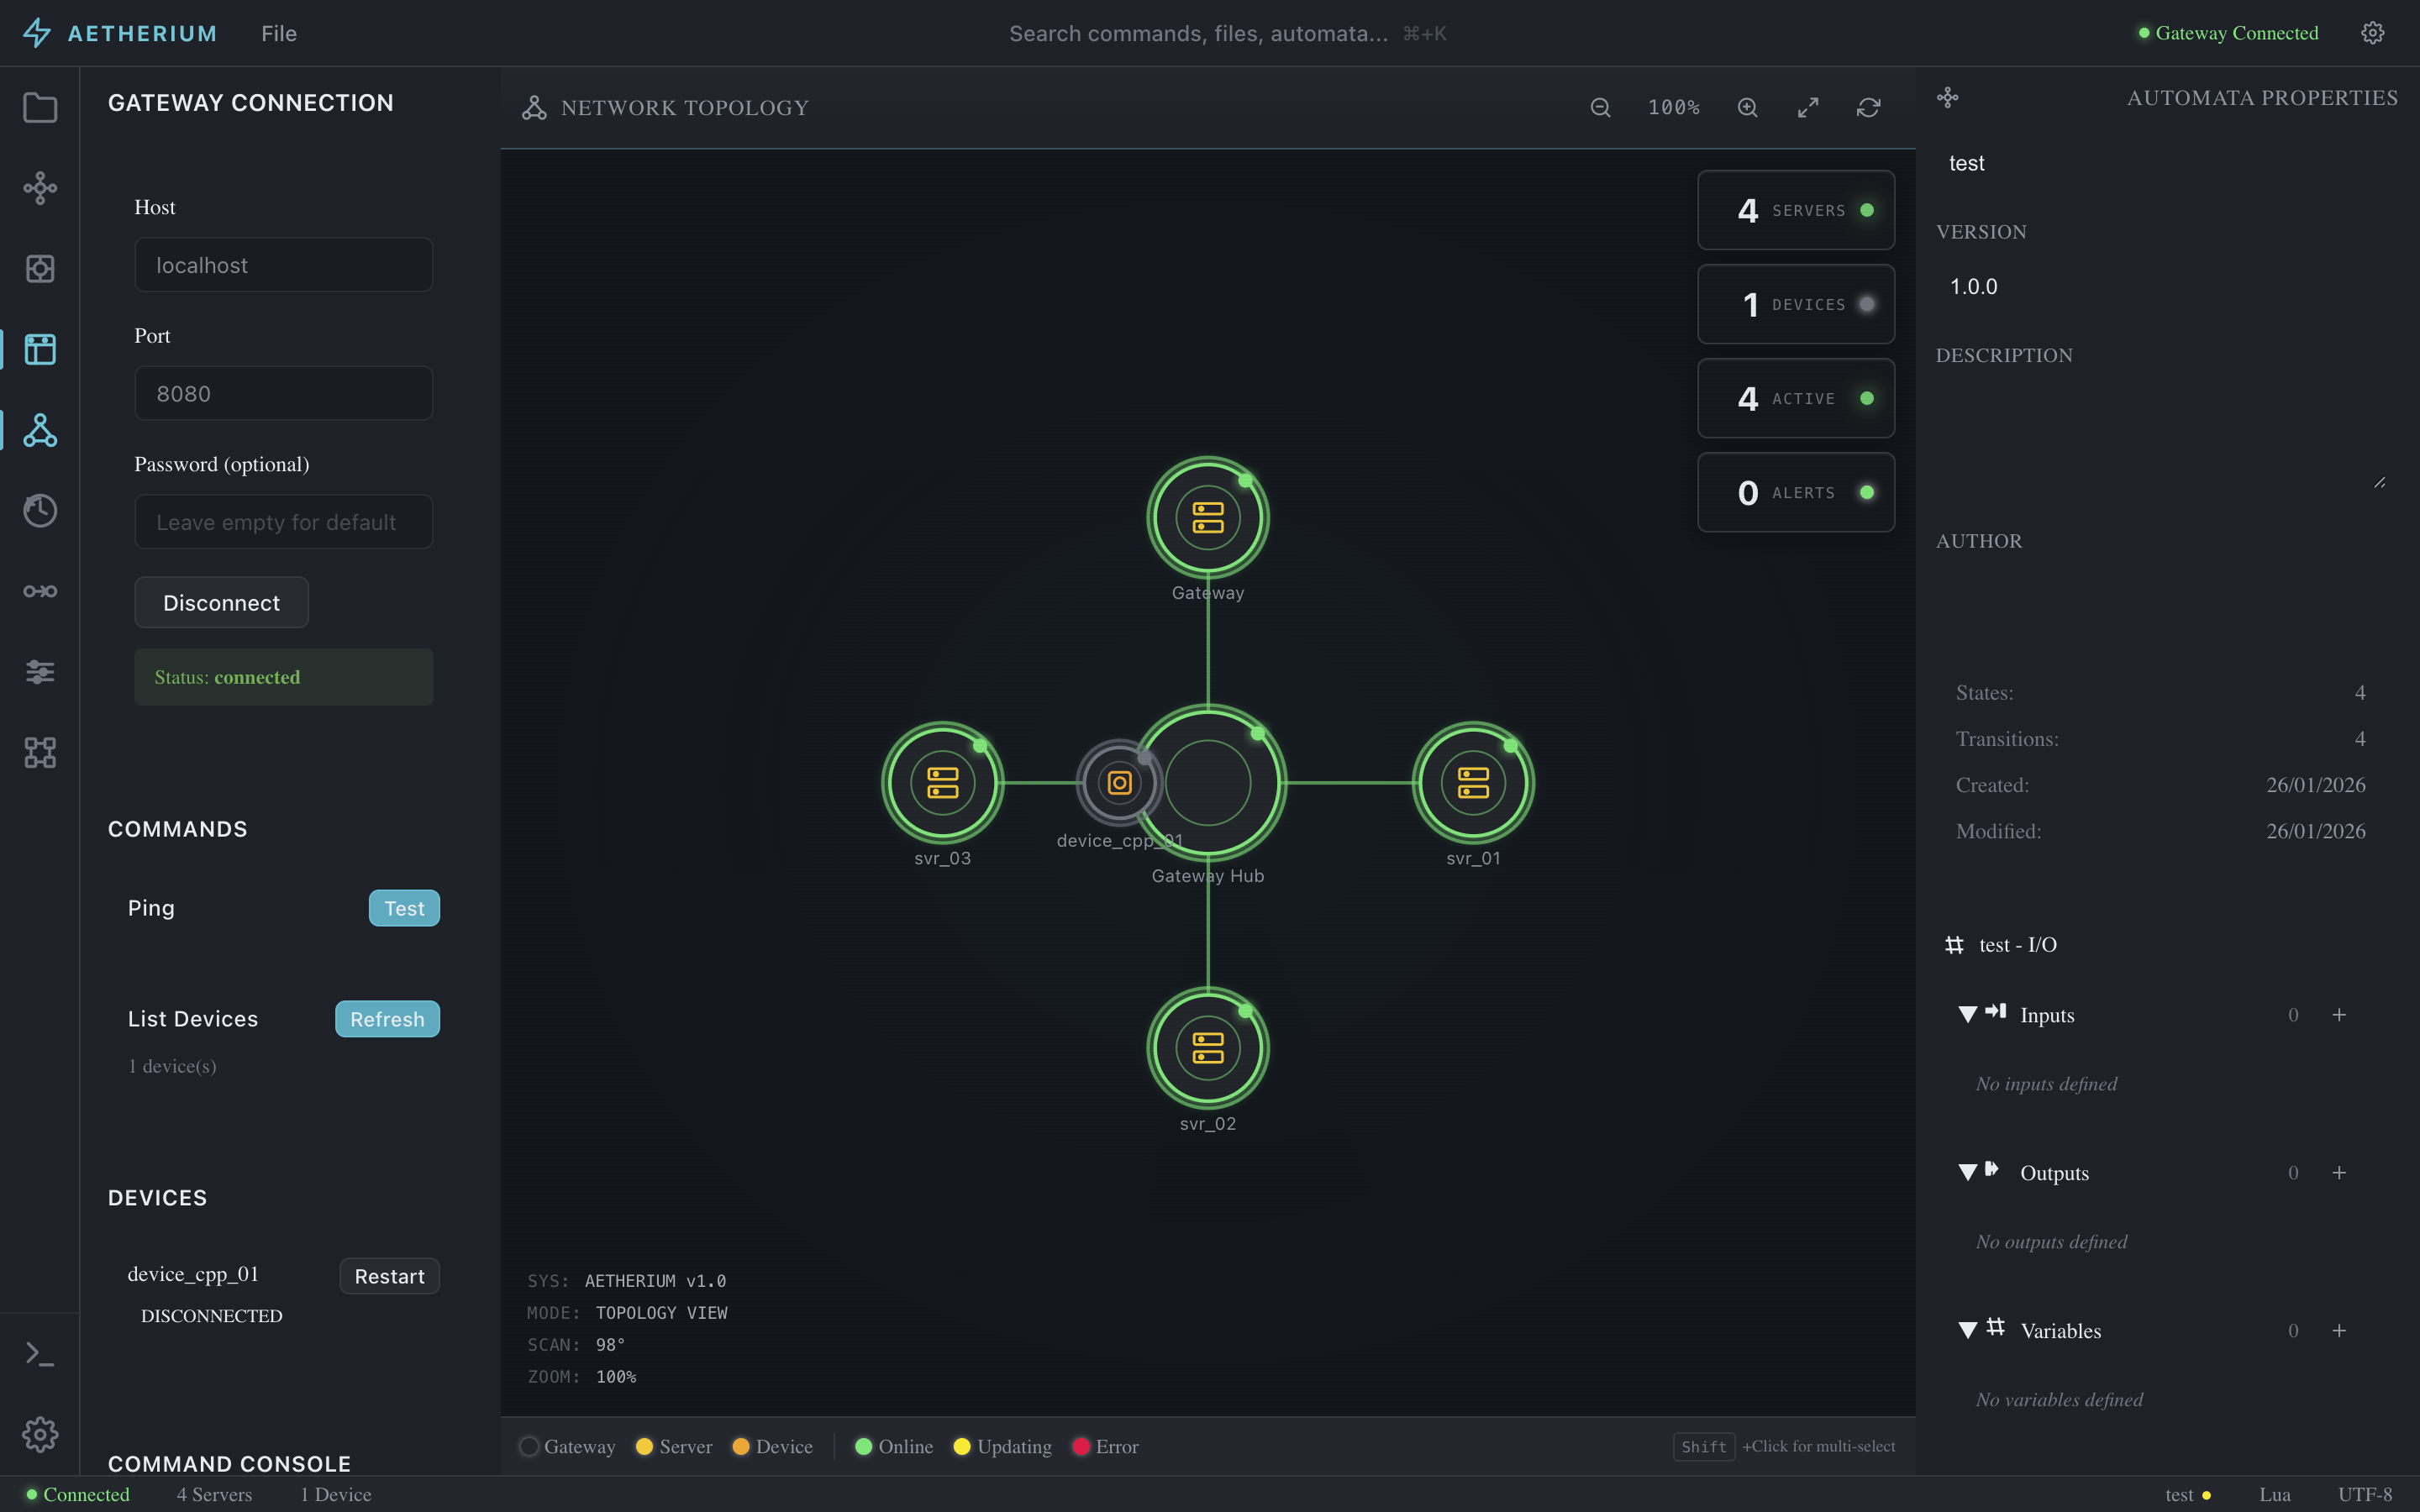
\includegraphics[width=\textwidth]{img/network.png}
  \end{columns}
\end{frame}


%%%%%%%%                       02 - Objectives                      %%%%%%%%
%---------------------------------------------------------------------------
% (Removed to keep the talk within 5 minutes and let the pictures drive.)


%%%%%%%%                      03 - Architecture                      %%%%%%%%
%---------------------------------------------------------------------------
\begin{frame}
  \frametitle{System Architecture (Current State)}
  \begin{columns}
    \column{0.44\textwidth}
    \begin{itemize}
        \item Timed automata run on multiple nodes.
        \item Gateway/server connect, coordinate, and observe.
    \end{itemize}

    \column{0.56\textwidth}
    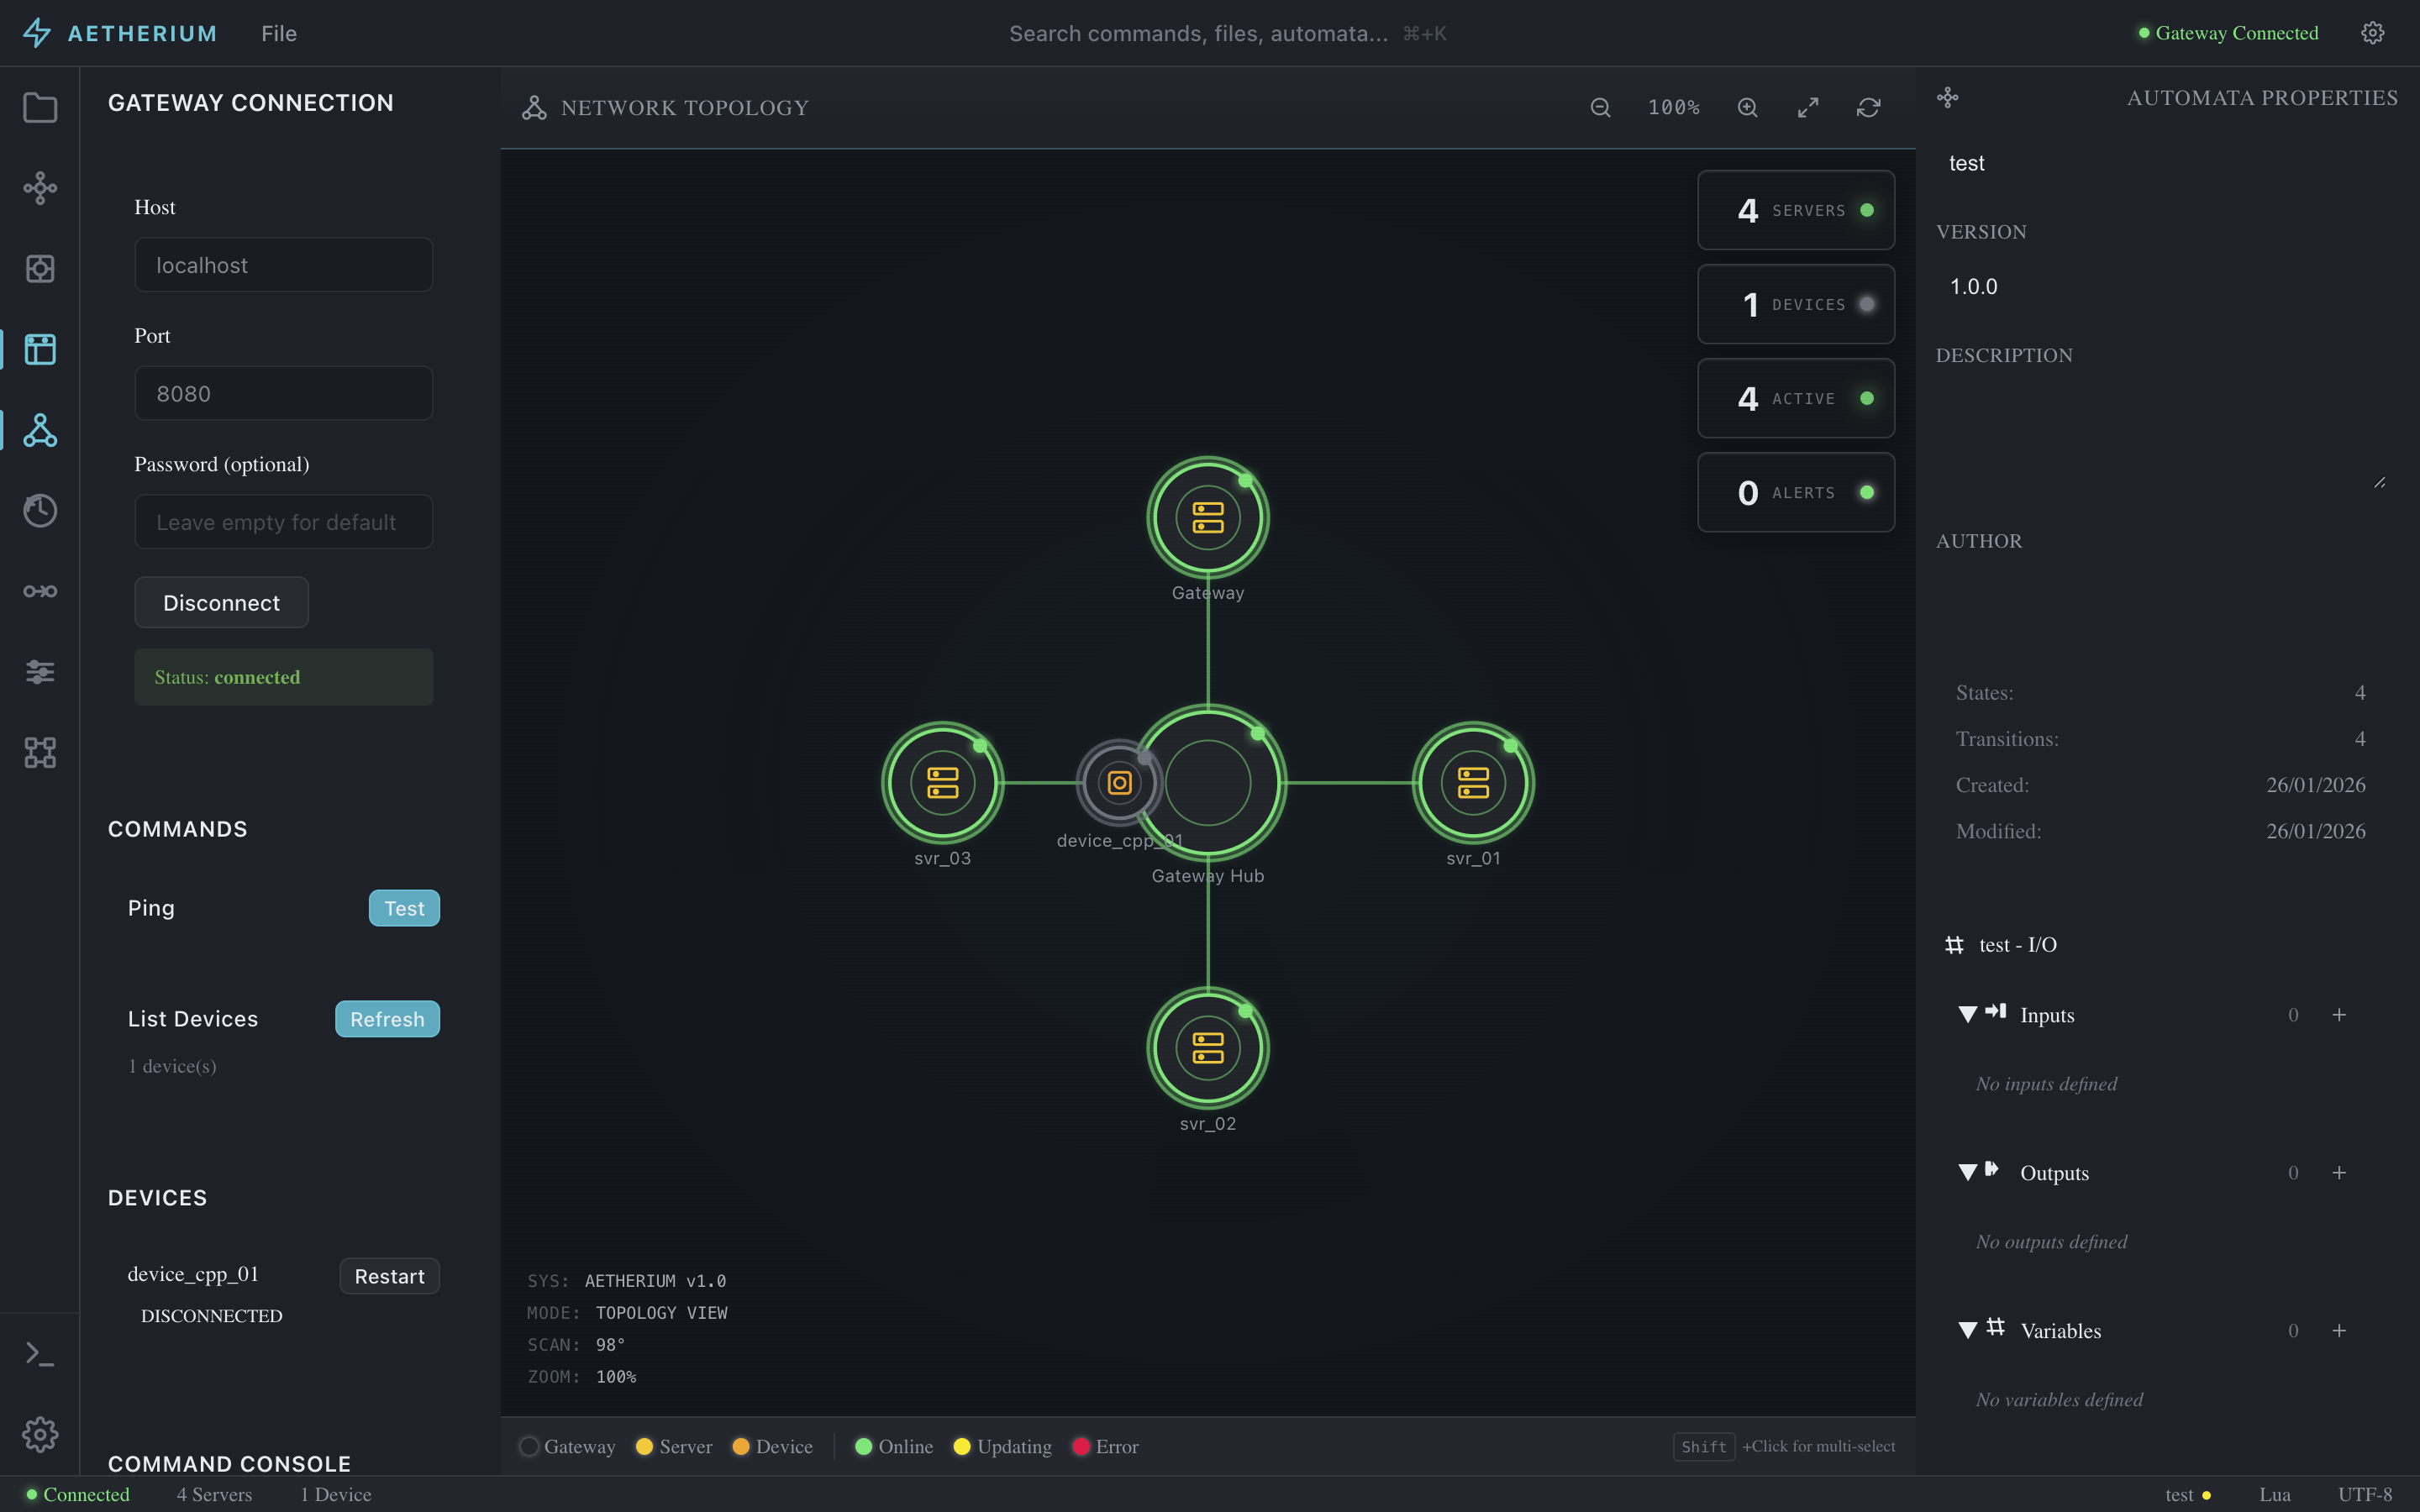
\includegraphics[width=\textwidth]{img/network.png}
  \end{columns}
\end{frame}

\begin{frame}
  \frametitle{Runtime: Timed Automata + Scripting}
  \begin{columns}
    \column{0.52\textwidth}
    \begin{itemize}
        \item YAML model: states, transitions, variables.
        \item Lua hooks for custom logic.
    \end{itemize}

    \column{0.48\textwidth}
    \includegraphics[width=\textwidth]{img/lua\_code.png}
  \end{columns}
\end{frame}


%%%%%%%%                        04 - Deployment                      %%%%%%%%
%---------------------------------------------------------------------------
\begin{frame}
  \frametitle{Deployment \,/\, Infrastructure (Current State)}
  \begin{columns}
  \column{0.52\textwidth}
    \begin{itemize}
      \item Docker-based services for repeatable development.
      \item Tested gateway/server + engine CLI.
    \end{itemize}
    
  \column{0.48\textwidth}
    \includegraphics[width=\textwidth]{img/docker\_showcase.png}
    
  \end{columns}
\end{frame}


%%%%%%%%                 05 - Finished Requirements                 %%%%%%%%
%---------------------------------------------------------------------------

\begin{frame}
  \frametitle{Finished Requirements (Summary)}
  \begin{itemize}
    \item \textbf{Studied:} DEVS, IEC~61499, Node-RED, 4diac/FORTE, ROS2/Micro-ROS.
    \item \textbf{Implemented / in progress:} runtime + protocol + services; IDE/time-travel/reconfiguration next.
  \end{itemize}
  \vspace{0.5em}
  \centering\includegraphics[width=0.82\textwidth]{img/time\_trave\_debugging.png}
\end{frame}


%%%%%%%%                        06 - Thanks                         %%%%%%%%
%---------------------------------------------------------------------------
% This slide should contain either one large or several smaller images arranged appropriately.
% Choose the best thing you want to show off - the committee will look at this slide the longest of all the slides.
% For this slide, thank the committee for attention (not necessarily by a huge text over the whole slide), and the committee will then have space to view the images as they listen to the reviews.
%---------------------------------------------------------------------------

% What is said at the end of the presentation is what the audience will consider when making subsequent decisions.

% HEROUT, Adam. Prezentování. Herout.net: Poznámky učitele, kouče, čtenáře. [online]. [cit. 2021-9-15]. Available at: https://www.herout.net/blog/category/prezentovani/
%---------------------------------------------------------------------------

\begin{frame}
  \frametitle{Thank You for Your Attention!}
  \centering
  \makebox[\textwidth]{\includegraphics[width=\paperwidth]{img/automata\_with\_transitions.png}}
\end{frame}

% Appendix removed: keep slide count low.